\documentclass[11pt,a4paper,oneside]{report}


\usepackage[T1]{fontenc}
\usepackage{times}

%==============================================================================
% GEOMETRY & SPACING
%==============================================================================

\usepackage[a4paper,margin=2.5cm]{geometry}

\usepackage{setspace}
\onehalfspacing

\setlength{\parskip}{0.5em}

%==============================================================================
% PACKAGE
%==============================================================================
\usepackage{tikz}
\usetikzlibrary{shapes.geometric, arrows.meta, positioning, fit, backgrounds}

\usepackage{graphicx}
\usepackage{amsmath}
\usepackage{amssymb}
\usepackage{amsfonts}
\usepackage{booktabs}
\usepackage{array}
\usepackage{tabularx}
\usepackage{longtable}
\usepackage{enumitem}
\usepackage{xcolor}
\usepackage{listings}
\usepackage{hyperref}
\usepackage{titlesec}
\usepackage{tcolorbox}
\usepackage{caption}


\renewcommand{\chaptername}{BAB}
\renewcommand{\contentsname}{DAFTAR ISI}
\renewcommand{\listfigurename}{DAFTAR GAMBAR}
\renewcommand{\listtablename}{DAFTAR TABEL}
\renewcommand{\appendixname}{LAMPIRAN}
\renewcommand{\figurename}{Gambar}
\renewcommand{\tablename}{Tabel}


\titleformat{\chapter}[display]
{\normalfont\Large\bfseries\centering}
{\chaptername\ \thechapter}
{12pt}
{\Large}

\titlespacing*{\chapter}{0pt}{-20pt}{20pt}

\hypersetup{
    colorlinks=true,
    linkcolor=black,
    urlcolor=black,
    citecolor=black,
    pdftitle={Progress Report - MK Kecerdasan Buatan}
}
\urlstyle{same}

%==============================================================================
% PETUNJUK BOX
%==============================================================================

\newtcolorbox{petunjuk}{
    colback=yellow!10,
    colframe=orange!60!black,
    boxrule=0.5pt,
    arc=2pt,
    left=6pt,
    right=6pt,
    top=4pt,
    bottom=4pt,
    fontupper=\small\itshape
}


\newcommand{\statusbox}[1]{
    \textbf{[STATUS: #1]}
}

%==============================================================================
% JSON STYLE
%==============================================================================

\lstdefinelanguage{json}{
    basicstyle=\ttfamily\footnotesize,
    showstringspaces=false,
    breaklines=true,
    frame=single,
    rulecolor=\color{gray!50},
    string=[s]{"}{"},
    stringstyle=\color{blue!60!black}
}

%==============================================================================
% DOCUMENT
%==============================================================================

\begin{document}

%==============================================================================
% COVER
%==============================================================================

\begin{titlepage}

\centering

\vspace*{1cm}

{\Large\bfseries PROGRESS REPORT \par}

\vspace{0.3cm}

{\large PROYEK PENGGANTI UAS \par}

\vspace{0.3cm}

{\large Mata Kuliah Kecerdasan Buatan \par}

{\large Semester Genap 2025/2026 \par}

\vspace{2cm}

{\LARGE\bfseries VisionGuard \par}

\vspace{0.5cm}

{\large Sistem Pendeteksi Kelelahan Pengemudi Kendaraan dengan \textit{Convolutional Neural Network} \par}

\vspace{2cm}

{\large Disusun oleh: \par}

\vspace{0.5cm}

\begin{tabular}{rl}
Benedict Aurelius & 2306209095\\
Deandro Najwan Ahmad Syahbanna & 2306213174 \\
Nelson Laurensius & 2306161845 \\
Wesley Frederick Oh & 2306202763 \\
\end{tabular}

\vspace{1.5cm}

{\large Dosen Pengampu: \par}

{\large Muhammad Firdaus Syawaludin Lubis, S.T., M.T., Ph.D. \par}

\vfill

{\large DEPARTEMEN TEKNIK KOMPUTER \par}

{\large FAKULTAS TEKNIK \par}

{\large UNIVERSITAS INDONESIA \par}

{\large 2026 \par}

\end{titlepage}

%==============================================================================
% TOC
%==============================================================================

\tableofcontents

\newpage

%==============================================================================
% EXECUTIVE SUMMARY
%==============================================================================

\chapter*{RINGKASAN EKSEKUTIF}

\addcontentsline{toc}{chapter}{Ringkasan Eksekutif}

Proyek ini dibuat dalam rangka pemenuhan tugas pada mata kuliah kecerdasan buatan sebagai tugas akhir. Proyek ini bertemakan \textbf{CNN} yang lebih berfokus pada pengembangan sistem pendeteksi kantuk pengemudi (Driver Drowsiness Detection atau DDD) sebagai upaya untuk menekan tingginya angka kecelakaan lalu lintas yang disebabkan oleh kelalaian manusia akibat mengantuk atau tidak fokus saat berkendara, khususnya kelelahan dan tertidur sesaat (\textit{micro sleep}). Untuk mengatasi keterbatasan sistem klasifikasi gambar global dengan model AI standar yang seringkali gagal pada kondisi tertentu seperti tingkat pencahayaan atau adanya fitur tertentu pada wajah, proyek ini mengimplementasikan arsitektur Faster Region-based Convolutional Neural Network (Faster RCNN). Pendekatan ini dipilih karena kemampuannya dalam melokalisasi fitur wajah secara presisi dan mengklasifikasikan kondisi pengemudi ke dalam empat kelas indikator biologis menggunakan dataset NTHU DDD.

Pada saat laporan \textit{progress report} ini disusun, status proyek telah mencapai persentase penyelesaian sebesar 50\%. Seluruh tahapan persiapan yang mencakup pengunduhan data, \textit{preprocessing}, penyesuaian format anotasi bounding box, hingga pengaturan arsitektur model telah berhasil diselesaikan. Saat ini, tim sedang berada pada fase \textit{training} model utama, dengan pemantauan loss function secara berkala guna memastikan model terhindar dari overfitting sebelum berlanjut ke fase evaluasi metrik akhir dan implementasi real time.

\vspace{0.5cm}

\noindent
\textbf{Persentase progres keseluruhan:} 50\%

%==============================================================================
% BAB 1
%==============================================================================

\chapter{PENDAHULUAN}

\section{Latar Belakang}

Penggunaan kendaraan pribadi, terutama di Indonesia, sangatlah populer dan menjadi alternatif utama daripada menggunakan kendaraan umum seperti kereta ataupun bus. Salah satu alasannya adalah pesatnya pertumbuhan pada mobilitas perkotaan seiring waktu dan perbaikan jalan di daerah perkotaan. 

Sebagian besar tingkat kecelakaan kendaraan darat yang terjadi banyak ditimbulkan akibat maraknya penggunaan kendaraan pribadi, yang terjadi akibat \textit{human error} dengan berbagai alasan lainnya seperti kelelahan pengemudi kendaraan dan kekurangan tidur menjadi faktor utama kecelakaan pada kendaraan pribadi. Pada daerah kota yang padat akan kendaraan, kelalaian pengendara manusia selama dua detik saja dapat menyebabkan kecelakaan yang sangat fatal. Di Indonesia pada tahun 2023 saja, dari 148.000 jumlah kecelakaan lalu lintas yang terjadi, 61\% darinya terjadi akibat faktor manusia seperti mengantuk, ceroboh, dan lain sebagainya \cite{b1}

Perkembangan dalam bidang \textit{computer vision} dan AI sangat memungkinkan untuk mengimplementasikan sistem \textit{camera-based Driver Drowsiness Detection} (DDD) \cite{b2} \cite{b3}. Namun, tantangan terbesar dalam aplikasi \textit{computer vision} saat berkendara adalah tingkat pencahayaan yang sangat bervariasi tergantung tempat dan waktu, baju/aksesoris yang digunakan seperti masker atau kacamata hitam, dan fitur muka yang sangat bervariasi tergantung etnis suku \cite{b4} \cite{b5}. Banyak model yang ada dilatih pada kumpulan data gambar statis yang sederhana yang gagal mereplikasi lingkungan dinamis yang kompleks ini, sehingga menyebabkan tingkat kesalahan positif yang tinggi dalam penerapan praktis.

Untuk mengatasi hal ini, kita akan menggunakan dataset NTHU Driver Drowsiness Detection (NTHU-DDD). Secara garis besar, dataset ini berisi tentang skenario-skenario gambar yang diambil dari beberapa video yang mencakup berbagai macam aspek, seperti kondisi pencahayaan dari yang gelap sampai ke terang, ekspresi dan keadaan psikologis pengendara, dan sebagainya.

Terlebih lagi, mengklasifikasikan seluruh \textit{frame} gambar sebagai mengantuk atau sadar/terbangun saja tidak memiliki presisi spasial yang dibutuhkan untuk sistem keselamatan yang dapat diaudit \cite{b6}. Oleh karena itu, proyek ini mengusulkan implementasi \textit{Faster Region-based Convolutional Neural Network} (Faster R-CNN). Dengan memanfaatkan \textit{Region Proposal Network} (RPN) terintegrasinya, Faster R-CNN unggul dalam melokalisasi titik-titik fokus pada tingkat kelelahan tertentu (misalnya, koordinat tepat mata yang terkulai atau mulut yang menguap) dalam latar belakang seperti kabin mobil \cite{b7} \cite{b8}. Hal ini memastikan bahwa prediksi kantuk terkait erat dengan fitur wajah pengendara yang sebenarnya, menghasilkan alur deteksi yang sangat akurat dan transparan.

\section{Rumusan Masalah}

\begin{enumerate}
    \item Model \textit{Driver Drowsiness Detection} (DDD) standar berbasis \textit{vision} mengalami penurunan akurasi ketika dihadapkan pada kondisi tertentu dunia nyata, yang mencakup aspek detail seperti tingkat pencahayaan atau adanya oklusi dan fitur-fitur wajah.
    \item Metode \textit{global image classification} tidak mampu menentukan koordinat presisi dari indikator kelelahan manusia, sehingga menyebabkan proses pengambilan keputusan AI menjadi tidak transparan dan sulit divalidasi.
    \item Terdapat kebutuhan krusial untuk mengevaluasi kinerja arsitektur object detection, secara spesifik Faster RCNN, dalam melokalisasi dan mengklasifikasi \textit{micro sleep} serta \textit{yawning} secara akurat menggunakan data sekuensial kompleks seperti dataset NTHU DDD.
\end{enumerate}

\section{Tujuan}
\begin{itemize}
\item Mengembangkan sistem \textit{vision-based Driver Drowsiness Detection} dengan memanfaatkan arsitektur Faster RCNN.
\item Melatih dan memvalidasi model menggunakan dataset NTHU DDD untuk memperbaiki tingkat \textit{resillience} model terhadap berbagai variasi faktor lingkungan, seperti perubahan pencahayaan siang malam serta penggunaan kacamata.
\item Mengevaluasi tingkat akurasi spasial model melalui akurasi bounding box beserta metrik klasifikasi, yang meliputi Precision, Recall, dan F1 Score, dalam membedakan antara perilaku mengemudi normal, \textit{yawning}, dan \textit{micro sleep}.
\item Membangun \textit{deployment pipeline} operasional yang sanggup menjalankan proses \textit{inference} pada \textit{video stream}, guna mendemonstrasikan kelayakan dan aplikabilitas praktis dari arsitektur yang diusulkan untuk skenario dunia nyata.
\end{itemize}

%==============================================================================
% BAB 2
%==============================================================================

\chapter{PENDEKATAN AI}

\section{Dataset}

Dataset yang digunakan pada proyek ini adalah \textbf{NTHU Driver Drowsiness Detection (NTHU-DDD) Multi-class} yang diperoleh dari repositori publik Kaggle. NTHU-DDD merupakan salah satu dataset tolok ukur (\textit{benchmark}) standar yang diakui dan secara luas digunakan untuk melatih serta mengevaluasi model \textit{computer vision} dalam mendeteksi kelelahan pada pengemudi. 

\subsection{Karakteristik Dataset}

Pada format aslinya, dataset NTHU-DDD terdiri dari rangkaian rekaman video. Namun, untuk keperluan proyek ini, kami menggunakan versi dataset yang telah diekstraksi ke dalam bentuk potongan \textit{frame} gambar berformat \texttt{.jpg}. Dataset ini sangat krusial untuk melatih model kecerdasan buatan karena dirancang secara khusus untuk merepresentasikan skenario berkendara di dunia nyata yang kompleks. Tingginya tingkat variasi pada dataset ini meliputi:

\begin{itemize}
    \item \textbf{Kondisi Pencahayaan (\textit{Illumination}):} Gambar diambil dalam kondisi siang hari (\textit{daylight}) dengan pencahayaan normal, maupun kondisi malam hari (\textit{nighttime}) yang menggunakan pencahayaan minim (seringkali memanfaatkan inframerah/NIR). Ini memaksa model untuk belajar mendeteksi fitur wajah tanpa bergantung sepenuhnya pada spektrum warna konvensional.
    \item \textbf{Aksesoris Pengemudi:} Terdapat variasi subjek pengemudi yang tidak menggunakan kacamata, menggunakan kacamata dengan efek pantulan cahaya (\textit{glare}), hingga subjek yang menggunakan kacamata hitam (\textit{sunglasses}). Variasi ini menjadi tantangan sekaligus melatih ketahanan (\textit{robustness}) model dalam mendeteksi kondisi mata.
    \item \textbf{Keragaman Subjek:} Dataset ini melibatkan banyak subjek yang berbeda-beda secara gender dan karakteristik wajah, yang berfungsi untuk meminimalkan risiko bias pada prediksi model akhir.
\end{itemize}

\subsection{Distribusi Kelas (Multi-class)}

Sesuai dengan nama \textit{multi-class} pada dataset, status pengemudi tidak hanya diklasifikasikan secara biner (mengantuk atau tidak), melainkan dibagi ke dalam beberapa kelas tindakan wajah (\textit{facial actions}) yang secara biologis mengindikasikan transisi menuju fase tertidur. Kelas-kelas tersebut meliputi:

\begin{enumerate}
    \item \textbf{Yawning (Menguap):} Kondisi di mana mulut pengemudi terbuka lebar melewati batas normal dalam durasi tertentu, yang menandakan penurunan kadar oksigen atau kelelahan.
    \item \textbf{Slow Blinking / Sleeping (Mata Terpejam):} Kondisi di mana kelopak mata subjek menutup dalam durasi yang lebih lama dari kedipan normal (\textit{microsleep}) atau tertutup sepenuhnya.
    \item \textbf{Nodding (Mengangguk):} Pergerakan gestur di mana kepala menunduk ke bawah secara tiba-tiba akibat otot leher yang rileks karena hilangnya kesadaran sesaat, lalu kembali tersentak ke atas.
    \item \textbf{Normal / Non-sleepy:} Kondisi \textit{baseline} di mana pengemudi sepenuhnya sadar, mata terbuka fokus ke depan, dan tidak menunjukkan tanda-tanda kelelahan.
\end{enumerate}

\subsection{Relevansi dengan Faster R-CNN}

Mengingat model yang kami kembangkan menggunakan arsitektur \textit{Faster Region-based Convolutional Neural Network} (Faster R-CNN), ketersediaan data gambar \texttt{.jpg} saja tidaklah cukup. Faster R-CNN bertindak sebagai \textit{object detector}, bukan sebatas pengklasifikasi gambar utuh. Oleh karena itu, kumpulan \textit{frame} dari dataset NTHU-DDD ini membutuhkan anotasi spasial berupa koordinat \textit{bounding box} (umumnya diatur dalam format \textit{Pascal VOC} atau \textit{COCO}). \textit{Bounding box} ini berfungsi untuk mengotakkan area \textit{Region of Interest} (RoI) pada bagian spesifik seperti wajah, mata, maupun mulut subjek, sehingga model dapat melokalisasi posisi dan mengenali kelas dari perilaku mengantuk tersebut.

\section{Model}

Pendekatan kecerdasan buatan yang digunakan dalam proyek ini berpusat pada arsitektur \textit{Faster Region-based Convolutional Neural Network} (Faster R-CNN). Faster R-CNN merupakan rumpun model \textit{two-stage object detector} yang diperkenalkan oleh Ren et al. (2015). Arsitektur ini dipilih karena memiliki keunggulan performa akurasi yang sangat tinggi dalam melokalisasi posisi objek dan mengenali kelas secara simultan, yang sangat krusial untuk mendeteksi area mikro pada wajah seperti kelopak mata dan bukaan mulut.

Secara garis besar, alur pemrosesan citra \texttt{.jpg} pengemudi di dalam model Faster R-CNN dibagi menjadi empat komponen utama, yaitu: \textit{Feature Extractor (Backbone)}, \textit{Region Proposal Network} (RPN), \textit{Region of Interest (RoI) Pooling/Align}, serta \textit{Classification \& Bounding Box Regression Head}. Alur struktural arsitektur ini diilustrasikan pada Gambar 2.1.

\begin{figure}[h!]
\centering

% Menyesuaikan ukuran diagram agar pas dengan lebar halaman
\resizebox{\textwidth}{!}{%
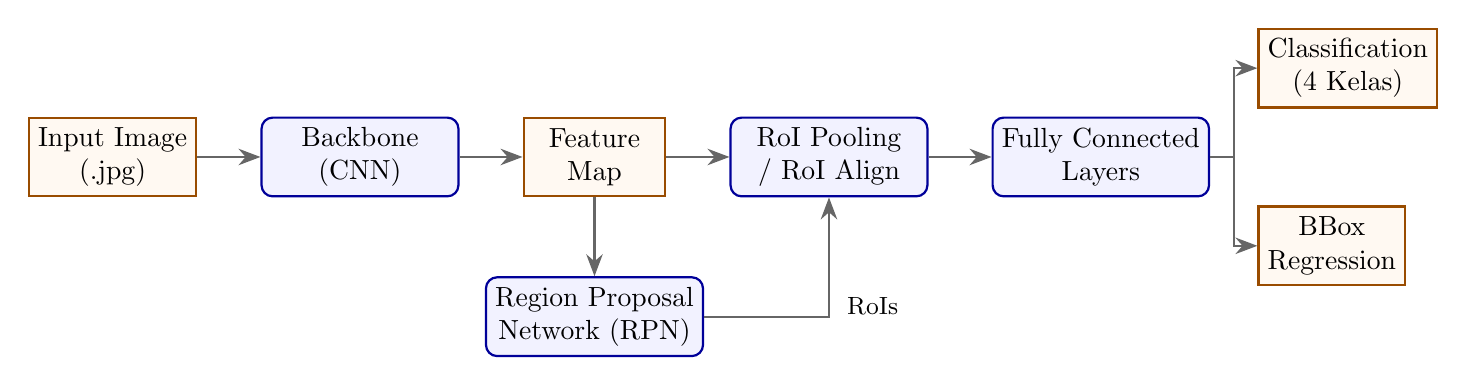
\begin{tikzpicture}[
    node distance=1cm and 0.8cm, % Jarak antar node dirapatkan
    % Mendefinisikan gaya untuk kotak (nodes)
    box/.style={rectangle, draw=blue!60!black, fill=blue!5, thick, minimum width=2.5cm, minimum height=1cm, align=center, rounded corners},
    io/.style={rectangle, draw=orange!60!black, fill=orange!5, thick, minimum width=1.8cm, minimum height=1cm, align=center},
    % Mendefinisikan gaya untuk panah
    arrow/.style={-{Stealth[scale=1.2]}, thick, draw=gray!80!black}
]

% Menempatkan Nodes (Kotak-kotak)
\node (input) [io] {Input Image\\(.jpg)};
\node (backbone) [box, right=of input] {Backbone\\(CNN)};
\node (featuremap) [io, right=of backbone] {Feature\\Map};
\node (roi) [box, right=of featuremap] {RoI Pooling\\/ RoI Align};
\node (fc) [box, right=of roi] {Fully Connected\\Layers};
\node (rpn) [box, below=of featuremap] {Region Proposal\\Network (RPN)};

\node (class) [io, above right=0.1cm and 0.6cm of fc] {Classification\\(4 Kelas)};
\node (bbox) [io, below right=0.1cm and 0.6cm of fc] {BBox\\Regression};

% Menghubungkan Nodes dengan Panah
\draw [arrow] (input) -- (backbone);
\draw [arrow] (backbone) -- (featuremap);
\draw [arrow] (featuremap) -- (roi);

% Panah dari Feature Map ke RPN
\draw [arrow] (featuremap) -- (rpn);

% Panah dari RPN ke RoI Pooling (menyampaikan RoIs)
\draw [arrow] (rpn.east) -| node[anchor=south west, xshift=0.1cm, yshift=-0.1cm] {\small RoIs} (roi.south);

% Panah ke FC dan Output
\draw [arrow] (roi) -- (fc);
\draw [arrow] (fc.east) -- ++(0.3,0) |- (class.west);
\draw [arrow] (fc.east) -- ++(0.3,0) |- (bbox.west);

\end{tikzpicture}%
} % akhir dari resizebox

\caption{Diagram Arsitektur Faster R-CNN untuk Deteksi Kantuk}
\label{fig:frcnn_diagram}
\end{figure}
\subsection{Backbone Network (Feature Extractor)}
Komponen pertama bertugas sebagai pengekstrak fitur dari gambar input \texttt{.jpg} mentah. Citra wajah pengemudi akan dilewatkan ke dalam jaringan konvolusi mendalam (\textit{Deep Convolutional Neural Network}) untuk mengubah matriks piksel gambar menjadi representasi fitur tingkat tinggi berbentuk \textit{feature map}. Fitur-fitur esensial seperti garis tepi mata, struktur bentuk bibir, dan orientasi kemiringan kepala akan terekstraksi pada tahap ini untuk diproses ke lapisan berikutnya.

\subsection{Region Proposal Network (RPN)}
RPN merupakan inovasi inti yang membedakan Faster R-CNN dari arsitektur pendahulunya (R-CNN dan Fast R-CNN). RPN bertindak secara efisien dengan memindai \textit{feature map} menggunakan mekanisme \textit{sliding window}. Di setiap posisi pindaian, RPN menghasilkan beberapa kandidat kotak pembatas yang disebut \textit{Anchor Boxes} dengan berbagai variasi skala (\textit{scale}) dan rasio aspek (\textit{aspect ratio}). 

RPN kemudian mengeluarkan dua jenis \textit{output}:
\begin{itemize}
    \item \textbf{Objectness Score:} Skor probabilitas apakah di dalam \textit{anchor box} tersebut terdapat objek (wajah/mata/mulut) atau hanya merupakan latar belakang (\textit{background}).
    \item \textbf{Bounding Box Regression:} Koordinat awal untuk menyesuaikan posisi \textit{anchor box} agar lebih pas membungkus objek target.
\end{itemize}
Kandidat terbaik dengan skor \textit{objectness} tertinggi akan dipilih sebagai \textit{Region Proposals} atau \textit{Region of Interest} (RoI).

\subsection{RoI Pooling / RoI Align}
Kandidat wilayah pembatas (RoI) yang dihasilkan oleh RPN memiliki ukuran dimensi (tinggi dan lebar) yang bervariasi. Di sisi lain, lapisan penciri akhir (\textit{Fully Connected Layer}) mensyaratkan vektor input yang berukuran tetap (\textit{fixed-size}). Lapisan \textit{RoI Pooling} atau \textit{RoI Align} bertugas untuk menjembatani perbedaan ini dengan melakukan pembagian wilayah RoI menjadi sub-grid tetap dan melakukan operasi \textit{max pooling} di dalamnya. Hasilnya adalah representasi fitur dengan ukuran seragam yang siap diklasifikasikan.

\subsection{Classification Head dan Bounding Box Regression}
Tahap akhir dari Faster R-CNN adalah melewatkan \textit{feature map} berukuran tetap dari proses \textit{RoI Pooling} ke dalam jaringan \textit{Fully Connected} (FC). Jaringan ini bercabang menjadi dua output linear (\textit{Multi-task Loss}):
\begin{enumerate}
    \item \textbf{Softmax Classifier:} Menghitung nilai probabilitas untuk menentukan kelas spesifik dari objek yang dideteksi di dalam \textit{bounding box}. Pada proyek ini, bagian ini akan mengklasifikasikan objek ke dalam salah satu dari 4 kategori indikator kantuk, yaitu \textit{Yawning}, \textit{Slow Blinking/Sleeping}, \textit{Nodding}, atau \textit{Normal}.
    \item \textbf{Bounding Box Regressor:} Menghitung pergeseran (\textit{offset}) numerik final ($x, y, w, h$) untuk menyempurnakan letak dan ukuran kotak pembatas akhir di sekitar wajah, mata, atau mulut pengemudi agar hasil deteksi spasialnya menjadi sangat presisi.
\end{enumerate}
%==============================================================================
% BAB 3
%==============================================================================

\chapter{PROGRES SAAT INI}

\section{Status Proyek}

Pada bab ini dipaparkan mengenai kemajuan atau progres dari pengerjaan proyek akhir pendeteksi kantuk (\textit{Driver Drowsiness Detection}) menggunakan model Faster R-CNN. Hingga saat laporan ini disusun, seluruh tahapan persiapan data gambar, penulisan kode arsitektur, hingga perancangan skrip \textit{training loop} telah berhasil diselesaikan secara penuh. Saat ini, fokus utama proyek berada pada fase komputasi intensif, yaitu proses pelatihan (\textit{training}) model awal.

Detail dari status capaian dan perkembangan masing-masing aktivitas proyek dapat dilihat pada Tabel 3.1.

\begin{table}[h!]
\centering
\begin{tabularx}{\textwidth}{lXl}
\toprule
Tahap & Aktivitas & Status \\
\midrule
Dataset & Pengunduhan dataset NTHU DDD dalam format \texttt{.jpg} & Selesai \\
EDA \& Splitting & Analisis distribusi gambar dan pembagian (\textit{train, validation, test set}) & Selesai \\
Preprocessing & Normalisasi gambar dan penyesuaian format anotasi \textit{bounding box} & Selesai \\
Arsitektur Model & \textit{Setup} arsitektur Faster R-CNN dan pembuatan berkas \textit{metadata} proyek & Selesai \\
Training & Eksekusi \textit{training loop} awal dan pemantauan \textit{loss function} & Berjalan \\
Evaluasi & Pengujian performa akhir model menggunakan metrik mAP & Belum \\
\bottomrule
\end{tabularx}
\caption{Status Proyek}
\end{table}

\section{Deskripsi Progres dan Kendala Pelatihan}

Berdasarkan garis waktu proyek pada tabel di atas, kelompok kami saat ini sedang memfokuskan sumber daya pada fase \textit{training} model Faster R-CNN. Seluruh blok kode program yang mencakup \textit{dataloader}, penentuan \textit{hyperparameter} (seperti \textit{learning rate} dan \textit{batch size}), serta alur \textit{training loop} utama telah selesai dirancang dan dapat dieksekusi dengan baik. 

Tantangan utama yang sedang dihadapi pada fase ini adalah durasi waktu komputasi yang cukup panjang. Karena Faster R-CNN merupakan arsitektur \textit{two-stage object detector} yang memproses ribuan file gambar \texttt{.jpg}, kalkulasi pada \textit{Region Proposal Network} (RPN) dan kepala klasifikasi memakan waktu yang signifikan di setiap \textit{epoch}. 

Proses monitoring dilakukan secara berkala terhadap pergerakan grafik \textit{loss function} (baik \textit{rpn loss} maupun \textit{roi loss}) pada \textit{training set} dan \textit{validation set}. Hal ini bertujuan untuk memastikan nilai \textit{loss} mengalami penurunan secara konvergen dan stabil, serta memastikan model tidak mengalami \textit{overfitting}.
%==============================================================================
% BAB 4
%==============================================================================

\chapter{KONTRIBUSI ANGGOTA}

\section{Wesley Frederick Oh (2306202763)}

\subsection*{Bagian yang Dikerjakan}
\begin{itemize}
    \item Penulisan laporan Bab 1: Pendahuluan.
    \item Eksplorasi Data (EDA) distribusi kelas pada dataset.
    \item Pembagian dataset (\textit{splitting}) menjadi \textit{train}, \textit{validation}, dan \textit{test set}.
\end{itemize}

\subsection*{Penggunaan AI Assistant}
\begin{itemize}
    \item Tool: Gemini
    \item Fungsi: Bantuan penyusunan draf narasi latar belakang dan perbaikan tata bahasa.
\end{itemize}

\section{Deandro Najwan Ahmad Syahbanna (2306213174)}

\subsection*{Bagian yang Dikerjakan}
\begin{itemize}
    \item Penulisan laporan Bab 2: Pendekatan AI.
    \item \textit{Preprocessing} dataset gambar \texttt{.jpg}.
    \item Penyesuaian format anotasi \textit{bounding box} agar kompatibel dengan model Faster R-CNN.
\end{itemize}

\subsection*{Penggunaan AI Assistant}
\begin{itemize}
    \item Tool: Gemini
    \item Fungsi: Pencarian referensi teori pendekatan AI dan \textit{formatting} dokumen.
\end{itemize}

\section{Benedict Aurelius (2306209095)}

\subsection*{Bagian yang Dikerjakan}
\begin{itemize}
    \item Penulisan laporan Bab 3 (Progres Saat Ini) dan Penulisan laporan Bab 4 (Kontribusi Anggota)
    \item Penulisan \textit{training loop} beserta pengaturan \textit{hyperparameter}.
    \item Eksekusi \textit{training} model Faster R-CNN dan pemantauan \textit{loss function}.
\end{itemize}

\subsection*{Penggunaan AI Assistant}
\begin{itemize}
    \item Tool: Gemini
    \item Fungsi: \textit{Debugging} kode PyTorch/\textit{framework} saat proses \textit{training} dan pemecahan \textit{error}.
\end{itemize}

\section{Nelson Laurensius (2306161845)}

\subsection*{Bagian yang Dikerjakan}
\begin{itemize}
    \item Penulisan laporan Bagian Metadata di Laporan Progress.
    \item \textit{Setup} Arsitektur Model.
    \item Pembuatan \textit{Metadata} proyek.
\end{itemize}

\subsection*{Penggunaan AI Assistant}
\begin{itemize}
    \item Tool: Gemini
    \item Fungsi: Bantuan penyusunan struktur \textit{metadata} (JSON) dan \textit{formatting} kode LaTeX.
\end{itemize}

%==============================================================================
% APPENDIX
%==============================================================================

\appendix

\chapter{Metadata}

\begin{lstlisting}[language=json]
{
  "kode_kelompok": "K02",
  "topik_pilihan": 1,
  "nama_topik": "Convolutional Neural Network (CNN)",
  "judul_proyek": "VisionGuard: Driver Drowsiness Detection menggunakan Faster R-CNN",

  "abstrak_singkat": "Proyek ini mengembangkan sistem Driver Drowsiness Detection (DDD) berbasis computer vision menggunakan arsitektur Faster R-CNN untuk mendeteksi kondisi kelelahan pengemudi secara real-time. Dataset utama yang digunakan adalah NTHU Driver Drowsiness Detection (NTHU-DDD) Multi-class dari Kaggle yang berisi berbagai kondisi pencahayaan, penggunaan aksesoris wajah, dan variasi perilaku pengemudi. Faster R-CNN dengan backbone ResNet50-FPN digunakan untuk melokalisasi dan mengklasifikasikan indikator kantuk seperti yawning, slow blinking, dan nodding menggunakan bounding box detection. Sistem dievaluasi menggunakan metrik object detection dan classification seperti Precision, Recall, F1-Score, dan mAP.",

  "metode_ai": [
    {
      "nama": "Faster R-CNN",
      "peran": "utama",
      "varian": "fasterrcnn_resnet50_fpn dengan pretrained COCO weights",
      "catatan": "Digunakan sebagai model utama object detection untuk mendeteksi indikator kantuk pengemudi."
    }
  ],

  "frameworks": [
    {
      "nama": "PyTorch",
      "versi": "2.2.2",
      "kegunaan": "Framework utama untuk training dan inference Faster R-CNN"
    },
    {
      "nama": "Torchvision",
      "versi": "0.17.2",
      "kegunaan": "Penyedia arsitektur Faster R-CNN dan preprocessing object detection"
    },
    {
      "nama": "OpenCV",
      "versi": "4.10",
      "kegunaan": "Image processing, HSV masking, dan bounding box extraction"
    },
    {
      "nama": "Albumentations",
      "versi": "1.4",
      "kegunaan": "Data augmentation dan preprocessing gambar"
    }
  ],

  "datasets": [
    {
      "nama": "NTHU Driver Drowsiness Detection Dataset (NTHU-DDD)",
      "tipe": "publik",
      "sumber": "Kaggle",
      "url_sumber_publik": "https://www.kaggle.com/datasets/samymesbah/nthu-dataset-ddd-multi-class",
      "jumlah_sampel": 0,
      "jumlah_kelas": 4,
      "proses_akuisisi_mandiri": "",
      "peran_di_proyek": "Dataset utama untuk training, validasi, dan evaluasi model Driver Drowsiness Detection.",
      "spek_rl": null
    },
    {
      "nama": "COCO Pretrained Weights",
      "tipe": "publik",
      "sumber": "PyTorch Torchvision",
      "url_sumber_publik": "https://pytorch.org/vision/stable/models/generated/torchvision.models.detection.fasterrcnn_resnet50_fpn.html",
      "jumlah_sampel": 0,
      "jumlah_kelas": 91,
      "proses_akuisisi_mandiri": "",
      "peran_di_proyek": "Bobot pretrained backbone Faster R-CNN untuk transfer learning.",
      "spek_rl": null
    }
  ],

  "metrik_utama": [
    "Precision",
    "Recall",
    "F1-Score",
    "mAP",
    "Confusion Matrix"
  ],

  "klaim_bonus": [""],

  "anggota": [
    {
      "nama": "Wesley Frederick Oh",
      "npm": "2306202763",
      "peran_utama": "Data Engineer & Documentation",
      "focus_area": [
        "Eksplorasi dataset",
        "Distribusi kelas",
        "Train-validation-test split",
        "Penyusunan laporan pendahuluan"
      ],
      "konsep_dikuasai_implementasi": [
        "Stratified dataset splitting",
        "EDA dataset citra",
        "Analisis distribusi kelas"
      ],
      "konsep_dikuasai_teori": [
        "Dataset imbalance",
        "Konsep Driver Drowsiness Detection",
        "Computer vision dataset preprocessing"
      ],
      "bagian_laporan": [
        "Bab 1"
      ],
      "bagian_kode": [
        "EDA dataset",
        "Dataset splitting"
      ]
    },

    {
      "nama": "Deandro Najwan Ahmad Syahbanna",
      "npm": "2306213174",
      "peran_utama": "Preprocessing & Annotation Engineer",
      "focus_area": [
        "Preprocessing citra",
        "Bounding box formatting",
        "Annotation processing",
        "Dataset preparation"
      ],
      "konsep_dikuasai_implementasi": [
        "Bounding box preprocessing",
        "HSV masking",
        "Annotation conversion",
        "Image preprocessing"
      ],
      "konsep_dikuasai_teori": [
        "Object detection annotation",
        "Bounding box representation",
        "Image preprocessing untuk CNN"
      ],
      "bagian_laporan": [
        "Bab 2"
      ],
      "bagian_kode": [
        "Bounding box generation",
        "Dataset preprocessing pipeline"
      ]
    },

    {
      "nama": "Benedict Aurelius",
      "npm": "2306209095",
      "peran_utama": "Model & Training Engineer",
      "focus_area": [
        "Training Faster R-CNN",
        "Training loop",
        "Hyperparameter tuning",
        "Loss monitoring"
      ],
      "konsep_dikuasai_implementasi": [
        "Faster R-CNN training",
        "Optimizer configuration",
        "Learning rate scheduling",
        "Training loop PyTorch"
      ],
      "konsep_dikuasai_teori": [
        "Region Proposal Network",
        "Transfer learning",
        "Backpropagation",
        "Loss convergence"
      ],
      "bagian_laporan": [
        "Bab 3",
        "Bab 4"
      ],
      "bagian_kode": [
        "Training loop",
        "Model training pipeline"
      ]
    },

    {
      "nama": "Nelson Laurensius",
      "npm": "2306161845",
      "peran_utama": "Metadata & Object Detection Pipeline Engineer",
      "focus_area": [
        "Metadata management",
        "Object detection pipeline",
        "Bounding box validation",
        "Model configuration",
        "Technical documentation"
      ],
      "konsep_dikuasai_implementasi": [
        "Class mapping management",
        "Bounding box validation",
        "Metadata JSON pipeline",
        "Object detection preprocessing",
        "Faster R-CNN configuration"
      ],
      "konsep_dikuasai_teori": [
        "Object detection workflow",
        "Bounding box coordinate system",
        "Metadata consistency",
        "Region-based object detection"
      ],
      "bagian_laporan": [
        "Metadata",
        "Bab 2.2"
      ],
      "bagian_kode": [
        "Metadata pipeline",
        "Bounding box validation",
        "Class mapping configuration",
        "Dataset metadata generation"
      ]
    }
  ],

  "tautan": {
    "github": "https://github.com/Deann7/FinalProject_CNN_Kel02_KecerdasanBuatan-01",
    "dataset_mandiri": null,
    "video_demo": null
  },

  "ai_assistant_usage": {
    "digunakan": true,
    "tools": [
      "Gemini"
    ],
    "bagian": [
      "Debugging environment PyTorch dan NumPy",
      "Penyusunan metadata JSON proyek",
      "Perbaikan struktur metadata dan object detection pipeline",
      "Review dokumentasi teknis Faster R-CNN",
      "Formatting LaTeX dan struktur laporan"
    ],
    "estimasi_persentase": 20
  }
}
\end{lstlisting}

%==============================================================================
% END
%==============================================================================
\renewcommand{\bibname}{Referensi}

\begin{thebibliography}{00}

\bibitem{b1} \url{https://goodstats.id/article/jumlah-tragedi-kecelakaan-di-indonesia-terus-meningkat-02jno}
\bibitem{b2} \url{https://pmc.ncbi.nlm.nih.gov/articles/PMC11819803/}
\bibitem{b3} \url{https://www.researchgate.net/publication/403598464_Deep_Learning-based_Driver_Drowsiness_Detection_and_Real-time_Alert_System}
\bibitem{b4} \url{https://www.mdpi.com/2076-3417/15/16/9018}
\bibitem{b5} \url{https://journals.plos.org/plosone/article?id=10.1371/journal.pone.0304669}
\bibitem{b6}  \url{https://www.researchgate.net/publication/404270092_Hybrid_YOLOv5s-faster_R-CNN_detector_for_complex_road-scene_object_detection}
\bibitem{b7} \url{https://www.digitalocean.com/community/tutorials/faster-r-cnn-explained-object-detection}
\bibitem{b8} \url{https://ieeexplore.ieee.org/abstract/document/10771046}

\end{thebibliography}

\end{document}